\documentclass[tikz]{standalone} 
\usetikzlibrary{decorations.pathmorphing,patterns}
%\renewcommand\familydefault{\sfdefault}

\usetikzlibrary{patterns}

\begin{document}
	
	%\tdplotsetmaincoords{0}{0}
	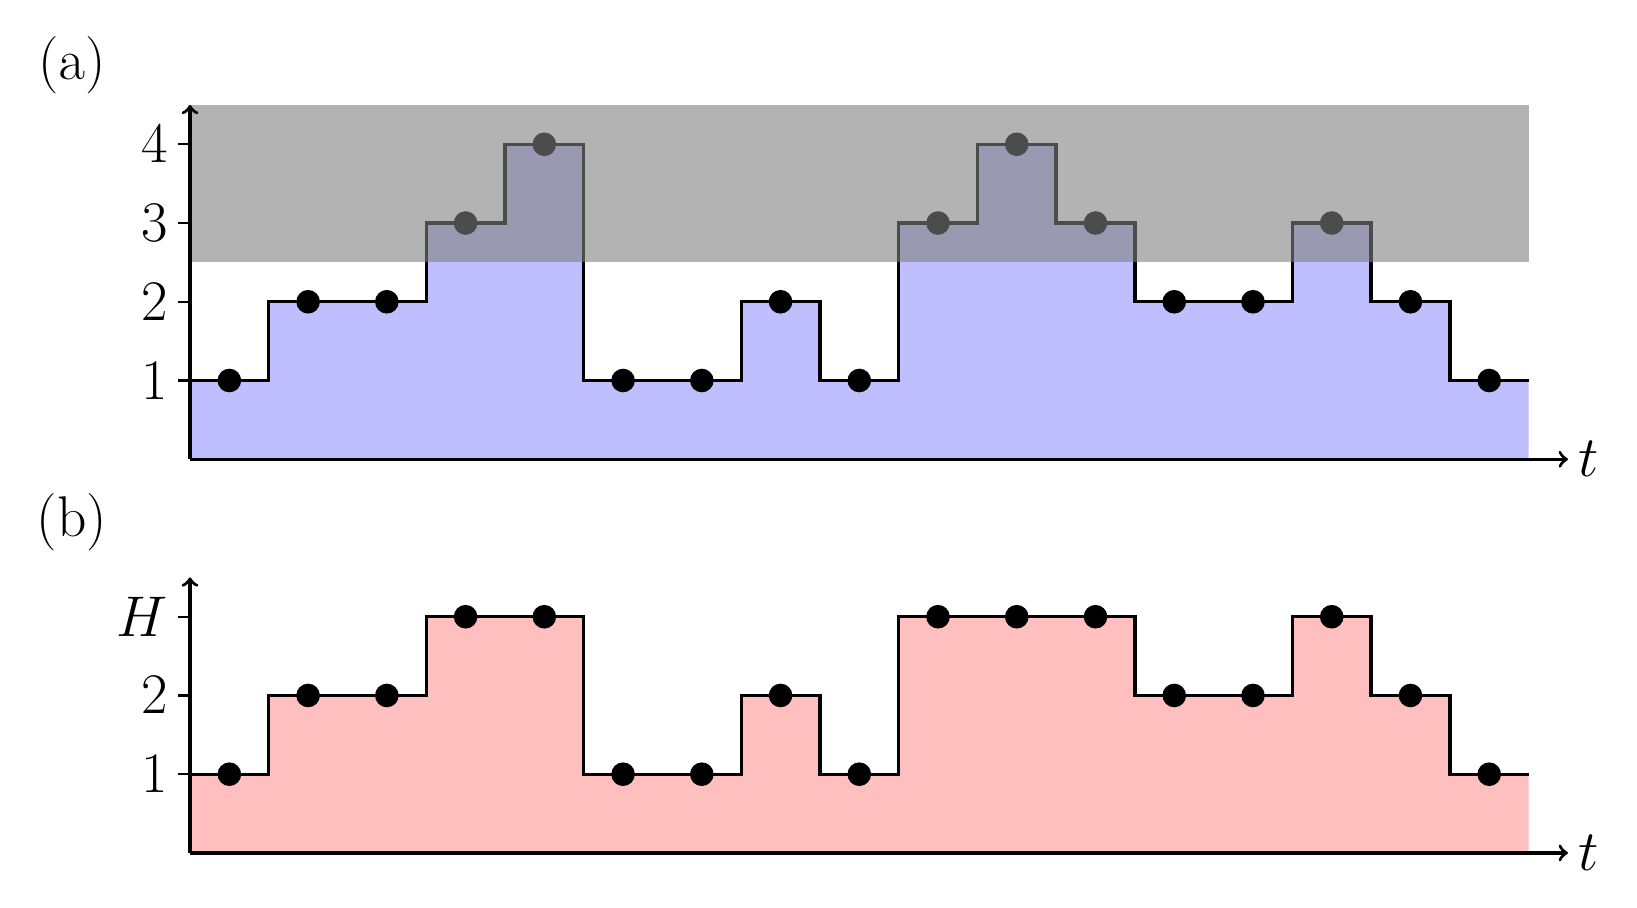
\begin{tikzpicture}
		\fill[blue!25] (0,0) to (0,1) to (1,1) to (1,2) to (3,2) to (3,3) to (4,3) to (4,4) to (5,4) to (5,1) to (7,1) to (7,2) to (8,2) to (8,1) to (9,1) to (9,3) to (10,3) to (10,4) to (11,4) to (11,3) to (12,3) to (12,2) to (14,2) to (14,3) to (15,3) to (15,2) to (16,2) to (16,1) to (17,1) to (17,0);
		\draw[thick] (-0.15 ,1)node[left]{\huge $1$} to (0,1);
		\draw[thick] (-0.15 ,2)node[left]{\huge $2$} to (0,2);
		\draw[thick] (-0.15 ,3)node[left]{\huge $3$} to (0,3);
		\draw[thick] (-0.15 ,4)node[left]{\huge $4$} to (0,4);
		\draw[very thick] (0,1) to (1,1) to (1,2) to (3,2) to (3,3) to (4,3) to (4,4) to (5,4) to (5,1) to (7,1) to (7,2) to (8,2) to (8,1) to (9,1) to (9,3) to (10,3) to (10,4) to (11,4) to (11,3) to (12,3) to (12,2) to (14,2) to (14,3) to (15,3) to (15,2) to (16,2) to (16,1) to (17,1);
		\fill (0.5,1) circle (0.15);
		\fill (1.5,2) circle (0.15);
		\fill (2.5,2) circle (0.15);
		\fill (3.5,3) circle (0.15);
		\fill (4.5,4) circle (0.15);
		\fill (5.5,1) circle (0.15);
		\fill (6.5,1) circle (0.15);
		\fill (7.5,2) circle (0.15);
		\fill (8.5,1) circle (0.15);
		\fill (9.5,3) circle (0.15);
		\fill (10.5,4) circle (0.15);
		\fill (11.5,3) circle (0.15);
		\fill (12.5,2) circle (0.15);
		\fill (13.5,2) circle (0.15);
		\fill (14.5,3) circle (0.15);
		\fill (15.5,2) circle (0.15);
		\fill (16.5,1) circle (0.15);
		\fill[gray,opacity=0.6] (0,2.5) to (0,4.5) to (17,4.5) to (17,2.5) to cycle;
		\draw[very thick,->] (0,0) to (17.5,0) node[right]{\huge $t$};
		\draw[very thick,->] (0,0) to (0,4.5);
		\draw[] (-1.5,5) node[]{\huge (a)};
		
		\begin{scope}[shift={(0,-5.0)}]
			\fill[red!25] (0,0) to (0,1) to (1,1) to (1,2) to (3,2) to (3,3) to (4,3) to (4,3) to (5,3) to (5,1) to (7,1) to (7,2) to (8,2) to (8,1) to (9,1) to (9,3) to (11,3) to (11,3) to (12,3) to (12,3) to (12,2) to (13,2) to (14,2) to (14,3) to (15,3) to (15,2) to (16,2) to (16,1) to (17,1) to (17,0);
			\draw[thick] (-0.15 ,1)node[left]{\huge $1$} to (0,1);
			\draw[thick] (-0.15 ,2)node[left]{\huge $2$} to (0,2);
			\draw[thick] (-0.15 ,3)node[left]{\huge $H$} to (0,3);
			\draw[very thick] (0,1) to (1,1) to (1,2) to (3,2) to (3,3) to (4,3) to (4,3) to (5,3) to (5,1) to (7,1) to (7,2) to (8,2) to (8,1) to (9,1) to (9,3) to (11,3) to (11,3) to (12,3) to (12,3) to (12,2) to (13,2) to (14,2) to (14,3) to (15,3) to (15,2) to (16,2) to (16,1) to (17,1);
			\fill (0.5,1) circle (0.15);
			\fill (1.5,2) circle (0.15);
			\fill (2.5,2) circle (0.15);
			\fill (3.5,3) circle (0.15);
			\fill (4.5,3) circle (0.15);
			\fill (5.5,1) circle (0.15);
			\fill (6.5,1) circle (0.15);
			\fill (7.5,2) circle (0.15);
			\fill (8.5,1) circle (0.15);
			\fill (9.5,3) circle (0.15);
			\fill (10.5,3) circle (0.15);
			\fill (11.5,3) circle (0.15);
			\fill (12.5,2) circle (0.15);
			\fill (13.5,2) circle (0.15);
			\fill (14.5,3) circle (0.15);
			\fill (15.5,2) circle (0.15);
			\fill (16.5,1) circle (0.15);
			\draw[very thick,->] (0,0) to (17.5,0) node[right]{\huge $t$};
			\draw[very thick,->] (0,0) to (0,3.5);
			\draw[] (-1.5,4.2) node[]{\huge (b)};
		\end{scope}
		
		
	\end{tikzpicture}
	
\end{document}